\chapter{Projektrisiken}
Im Risikomanagement werden folgende Fragen geklärt:

\begin{itemize}
	\item Wohin läuft das Projekt?
	\item Welche Risiken und Unsicherheiten gibt es?
	\item Wie können diese beherrscht werden?
	\item Wie gehen wir mit sich ändernden Anforderungen um?
	\item Was müssen wir heute anders entscheiden, damit wir morgen mit unserem Projekt erfolgreich sind?
\end{itemize}

In vielen Unternehmen wird eine Kultur der Brandstifter gelebt. Es wird ein Brand gelegt, dieser wird unter grossen Einsatz gelöscht und dann wird man dafür ausgezeichnet. Besser ist aber eine Kultur in der Vorsorge belohnt wird.

\section{Sie können den Begriff des Risikos definieren und erläutern, mit welchen Methoden Risiken identifiziert werden können.}
\label{sec:risikomanagement-definition-risiko}

Ein Risiko ist ein unsicheres Ereignis mit negativen Auswirkungen. Risiko des Einen, Chance des Anderen. Kein Geschäftserfolg ohne Risiko. Risiken und Nutzen wachsen oft proportional.

\begin{center}
	\begin{math}
		Risiko = Eintrittswahrscheinlichkeit \times Auswirkung
	\end{math}
\end{center}

\paragraph{Vorgehen}
\begin{enumerate}
	\item Risiken identifizieren
	\item Risiken bewerten
	\item Risiken abschwächen
	\item Risiken verfolgen 
\end{enumerate}
Risiken können in die folgenden Arten unterteilt werden:
\begin{itemize}
	\item Technische Risiken
		\subitem Zu wenig Know-How zu einer Technologie
		\subitem Technische Spezifikationen von Produkten nicht korrekt
		\subitem Termintreue und Qualität von Lieferanten
		\subitem Patente von Mitbewerbern
	\item Implementierungsrisiken
		\subitem Anforderungen ändern sich oder Konflikte nicht aufgelöst
		\subitem Architektur \& Design falsch
		\subitem Entwicklungsprozess wird nicht beherrscht
	\item Wirtschaftliche \& Industrielle \& Geschäftsrisiken
		\subitem Ressourcen stehen nicht zur Verfügung
		\subitem Änderungen am Markt
		\subitem Mitbewerber haben bessere Produkte
		\subitem Verlust an kritischem Know-How durch Mitarbeiterfluktuation
\end{itemize}

\subsection{Identifzieren}
\begin{description}
	\item[Brainstorming] (immer) schnell, einfach, kann viele Risiken liefern. Jedoch systematische Fehler durch Gruppendruck, Vorurteile usw.
	\item[SWOT Analyse] (in komplexen Projekten) Projekt aus Sicht der übergeordneten Organisation betrachten. Stärken/Schwächen einer Organisation. Hilft, strategische Risiken zu identifizieren. Jedoch aufwendiger, ist der objektive Blickwinkel gegeben?
	\item[Bedrohungsszenarien] (bei konkreten Bedrohungen) Was wäre wenn? Situationen durchspielen, sind aber alle Situationen gefunden?
	\item[Übertragung von früheren Erfahrungen] (immer) Erfahrungen wiederverwenden. Aus Fehlern lernen. Konstruktive Analyse- und Lernbereitschaft vorhanden?
	\item[Interviews] (in komplexen Projekten) Identifikation von unklarer Schnittstellen und Erwartungen. Zeitaufwendig!
	\item[Konfliktanalyse] (bei konkreten Bedrohungen) Betrachtung von Interessensphären und Zielkonflikten. Beziehungen/Ziele von Schlüsselpersonen. Identifikation von WIN-WIN Situationen für Beteiligte. Anspruchsvoll, guter Kommunikationsstil nötig!
	\item[Checklisten] (immer) Erfahrungswesen aus der Literatur und der Branche. Einfach, Best Practices, geben Orientierung. Wie gut ist die Qualität der Liste?
	\item[Werkzeuge] Automatisierung systematischer Befragungen/Checklisten. Folgefragen in Abhängigkeit von Antworten. Automatische Auswertung. Nicht so einfach verfügbar!
\end{description}

Bei der Identifikation der Risiken fasst man diese in einer Tabelle zusammen. Man kann diese kategorisieren nach \textbf{Personen}, \textbf{Produkt}, \textbf{Prozess} und \textbf{Technologie}.

Top 5 der Risiken in Software-Projekten: 
\begin{enumerate}
	\item Ändernde Anforderungen
	\item Schlechte Benutzerschnittstelle
	\item Unzureichende Systemqualität
	\item Unrealistische Zeit- und Budgetplanung
	\item Technologieüberforderung oder unausgereifte Technologie
\end{enumerate}
	
\section{Sie kennen das Ziel und die wichtigsten Aufgaben des Risikomanagements.}

\paragraph{Ziele}
\begin{itemize}
	\item Potentielle Probleme erkennen bevor sie auftreten.
	\item Massnahmen ergreifen und durch gesamten Projektlebenszyklus durchführen, damit diese Probleme nicht auftreten und Projektziele gefährden.
	\item Risiken kontrollieren, nicht vermeiden.
	\item Frühzeitig und proaktiv an den Ursachen der wichtigsten Risiken eingreifen.
\end{itemize}

\paragraph{Aufgaben}
Siehe dazu die Liste Vorgehen in Abschnitt \ref{sec:risikomanagement-definition-risiko}


\section{Sie kennen Methoden zur Bewertung und Abschwächung von Risiken}

\subsection{Bewertung von Risiken}

Man muss das Risiko quantifizieren um diese vergleichen zu können. Die Risikobewertung sollte nie alleine durch Schlüsselpersonen wie der PL oder Projektowner erfolgen. Am besten zieht man sich ein externes Team hinzu. Oder von unabhängigen Gruppen identifizieren zu lassen. Zuerst ein Beispiel eines festgehaltenen Risikos:
\vfill
\begin{tabular}{|p{7cm}|p{7cm}|}
	\hline Risikoauslösendes Ereignis &  den Würfel werfen \\ 
	\hline Risiko & Geld verlieren, falls keine 6  \\ 
	\hline Eintrittswahrscheinlichkeit & 83 Prozent \\ 
	\hline Auswirkung & 10 CHF verloren \\ 
	\hline 
\end{tabular}

Eine Möglichkeit ein Risiko zu schätzen ist die einfache Risiko Quantifizierung. Dabei geht es darum, jedem Risiko einen Zahl von 1-5 zu geben. Risiko mit dem Gewicht von 5 ist katastrophal und Risiko mit dem Gewicht von 1 ist vernachlässigbar. Zudem gibt es noch folgende Schätzmethoden:
\begin{itemize}
	\item Finanzielle Schätzmethoden: NPV und diskontierter Cash Flow (siehe Business Case)
	\item \textbf{PERT/Dreipunktschätzung: (w(pessim)) + 4 x w(realist) + w(optimist)) / 6}
	\item Machbarkeitsstudie
	\item ABC Analyse
	\item Delphi-Methode
	\item Expertenschätzung
\end{itemize}
Abbildung \ref{fig:risiko-management-beispiel-berechnung} zeigt wie das Risiko zusätzliche Tests einsetzen in einem Softwareprojekt bewertet wird.
\begin{figure}[h!]
\centering
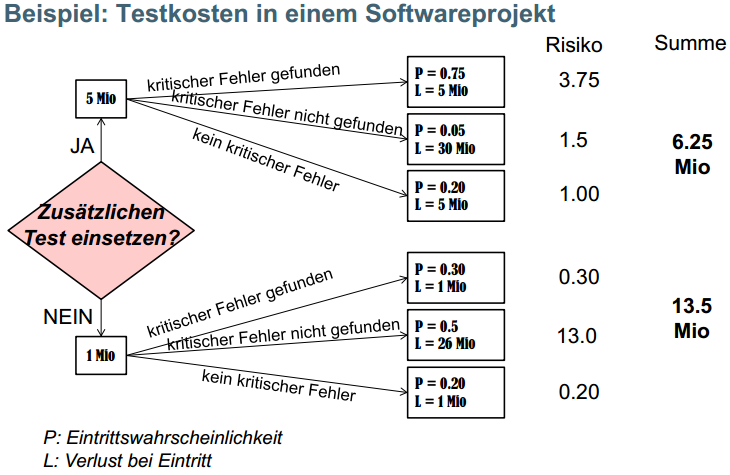
\includegraphics[width=0.7\linewidth]{fig/risiko-management-beispiel-berechnung}
\caption{Risikomgmt. Beispiel Berechnung}
\label{fig:risiko-management-beispiel-berechnung}
\end{figure}
Abbildung \ref{fig:risiko-management-muster-risiko-beschreibung} zeigt ein Muster für die Beschreibung eines Risikos.
\begin{figure}[h!]
\centering
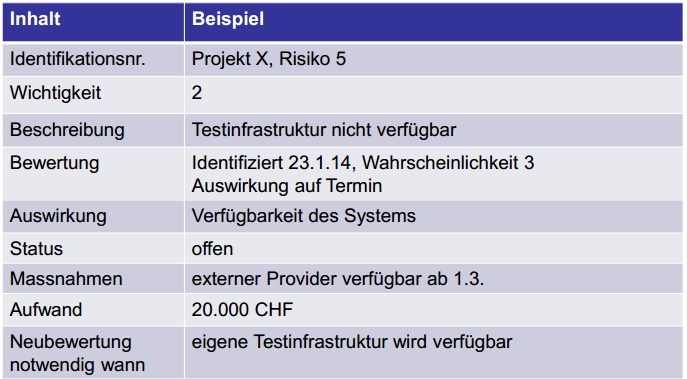
\includegraphics[width=0.8\linewidth]{fig/risiko-management-muster-risiko-beschreibung}
\caption{Risiko Management: Muster Risiko Beschreibung}
\label{fig:risiko-management-muster-risiko-beschreibung}
\end{figure}

\subsection{Abschwächung von Risiken}

Um ein Risiko abzuschwächen gibt es vier Möglichkeiten:
\begin{description}
	\item[Vermeiden] Eintrittswahrscheinlichkeit reduzieren. Man verzichtet so aber auch auf die Chance die das Risiko bietet.
	\item[Begrenzen] Auswirkung abschwächen. Wie bei einer Versicherung mit Selbstbeteiligung.
	\item[Behandeln] Durch zusätzlichen Aufwand Eintrittswahrscheinlichkeit und/oder Auswirkung reduzieren.
	\item[Ignorieren] Man lässt den Dingen seinen Lauf\dots
\end{description}
Abbildung \ref{fig:risiko-management-beispiel-abschwaechen-risiko} zeigt Massnahmen welche in den verschiedenen Kategorien ergriffen werden können um das Risiko abzuschwächen.
\begin{figure}[h!]
\centering
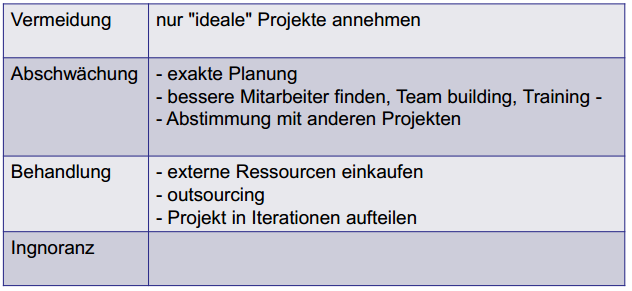
\includegraphics[width=0.7\linewidth]{fig/risiko-management-beispiel-abschwaechen-risiko}
\caption{Abschwächen des Risikos: Unzureichende Projektressourcen}
\label{fig:risiko-management-beispiel-abschwaechen-risiko}
\end{figure}
Risiken können auf mehreren Ebenen abgeschwächt werden:
\begin{description}
	\item[Innerhalb des Projekts] Frühzeitig sichtbare Risiken, die leicht abgeschwächt werden z.B. unklare Anforderungen, Fehler im Code usw. (Auf Ebene Meilenstein, AP).
	\item[Auf Projektebene] Spät sichtbare Risiken z.B. Integration von Komponenten, Abnahmen durch Kunden.
	\item[Für das gesamte Projekt] Sporadisch eintretende Risiken mit grösseren Auswirkungen z.B. Ressourcenmangel, Ausfall von Mitarbeitern.
\end{description}

Nach dem Risiken identifiziert, bewertet und abgeschwächt wurden, geht es darum, die Risiken auf dem Radar zu behalten. Nur Risiken die man aktiv verfolgt, verlieren Gefahrenpotential. Die vereinbarten Aktionen zur Abschwächung müssen überwacht werden. Greifen diese Aktionen zur Abschwächung? Hat sich die Bewertung geändert? Sind Risiken zu Probleme geworden? 

Bei mangelhaften Risikomgmt. entsteht oft folgendes: Feuerwehreinsätze (Risiken werden zu Problemen), unzufriedene Kunden (zu spät / zu teuer), teures Nacharbeiten, keine Systematik, keine Disziplin.
Abbildung \ref{fig:risiko-management-prozess} zeigt nochmal den gesamten Prozess des Risikomanagements zusammengefasst. Zudem ist auch die Kommunikation der Risiken (intern/extern) und die frühe Abschwächung (Projektstart) von Risiken wichtig.

\begin{figure}
\centering
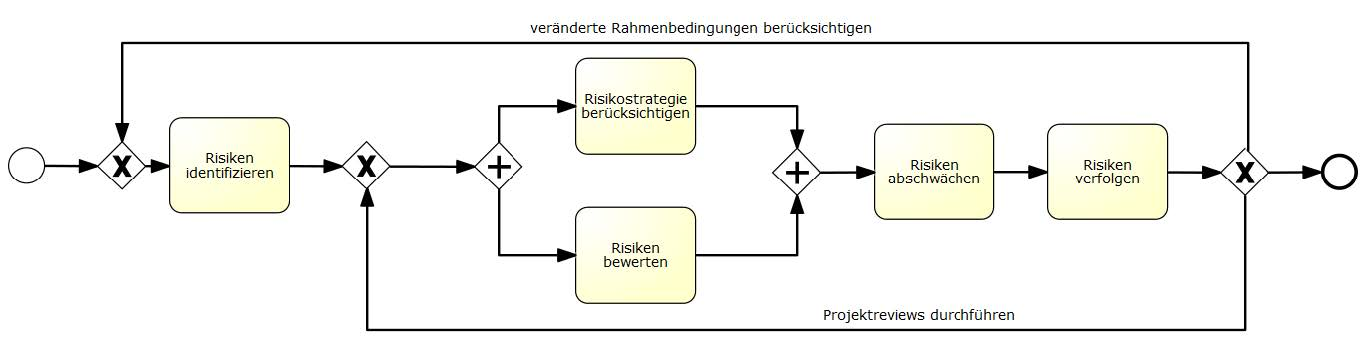
\includegraphics[width=0.7\linewidth]{fig/risiko-management-prozess}
\caption{Prozess des Risikomanagements}
\label{fig:risiko-management-prozess}
\end{figure}
 